\documentclass{article}
\usepackage{hw_style}
\usepackage{enumerate}
\usepackage{graphicx}
\usepackage{verbatim}

% Homework Specific Information
\newcommand{\hmwkTitle}{Homework \#2}
\newcommand{\hmwkDueDate}{Tuesday Oct. 18th}
\newcommand{\hmwkAuthorName}{Kurt Rudolph}%Name:
\newcommand{\hmwkNetID}{rudolph9}%your netid
\newcommand{\hmwkNotes}{}%I worked with...

\newcommand{\hmwkSubTitle}{}
\newcommand{\hmwkClass}{CS 412}
\newcommand{\hmwkClassTime}{Wed, Fri 3:30PM - 4:45PM}
\newcommand{\hmwkClassInstructor}{Jiawei Han}

\begin{document}
\begin{spacing}{1.1}
\maketitle
%=============================Problem1=========================%
\newpage
\begin{homeworkProblem}
	We model the users in a social network as a data cube. Suppose each user has 10 dimensions of information, such as age, gender, city and income. Assume a base cuboid of 10 dimensions contains three base cells: (1) ($b1, b2, a3, a4, a5, \dots, a9, a10):count=10, (2) (b1, a2, b3, a4, a5, \dots, a9, a10):count=20$, and $(3) (a1, b2, b3, a4, a5, \dots, a9, a10$):count=50, where $a_i != b_i, a_i!=a_j$, etc. The count measure of the cube means the number of users who satisfy such information.
	
	\begin{enumerate}[(1)]
		\item How many nonempty cuboids will a full data cube contain?
			\begin{homeworkSection}{Solution}
				\[2^{10} - 1 = 1023 \]
			\end{homeworkSection}
		\item How many nonempty aggregate (i.e., non-base) cells will a full cube contain?
			\begin{homeworkSection}{Solution}
				\[ totalCells - (overlappingCells * overlappingTimes) \]
				\[ = totalCells - (overlapTwiceCells*2 + overlapOnceCells*1 + baseCells) \]
				\[ =  3 * 2^{10} - (2^7*2 + 2^7*3*1 + 3) =   2429 \]
			\end{homeworkSection}
		\item How many nonempty aggregate cells will an iceberg cube contain if the condition of the iceberg cube is "$count \ge 70$"?
			\begin{homeworkSection}{Solution}
				Since one base cell has $count = 20$ and one base cell has $count = 70$ we simply need to compute the number of instances where subsets of these two base cells overlap, using our calculations from the previous problem we find: 
				\[ 27 *2+27 *3*1 = 135 \]
			\end{homeworkSection}
		\item How many closed cells are in the full cube? 
			\begin{homeworkSection}{Solution}
				There are 4, the three base cell and $(*,*,*,a4, a5, \dots, a9, a10)$.  
			\end{homeworkSection}
	\end{enumerate}
\end{homeworkProblem}
%=============================Problem2==========================%	
\newpage
\begin{homeworkProblem}
	Given the following base cuboid with count as the measure.\\
	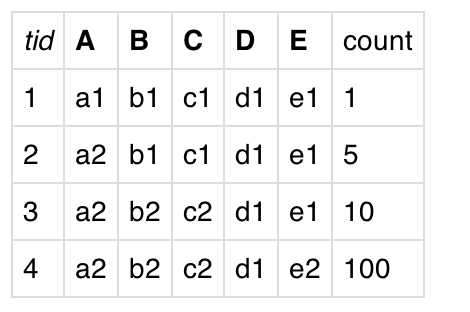
\includegraphics[width=2.5in]{prob2.png}
	\begin{enumerate}[(1)]
		\item Briefly outline the major steps to compute Shell-Fragment cube (refer to VLDB04 paper �High-Dimensional OLAP: A Minimal Cubing Approach�), suppose we divide the 5 dimensions into 2 shell fragments: AB and CDE.
			\begin{homeworkSection}{Solution}
				The major steps to compute Shell-Fragment cube start with vertically partitioning the high dimensional dataset in a set of disjoint low dimensional datasets (i.e. our two fragments AB and CDE).  For each of the fragments we compute its local data cube.  Next we register the set of tuple-ids that contribute to the non-empty cells in the fragment data cube.  These are used to bridge the gap between various garments and re-construct the corresponding cuboids upon request.  Essentially the data cubes of the original high diminutional space are dynamically assembled together view these fragments.  
			\end{homeworkSection}
		\item Briefly describe how to compute subcube query (a2,b2,*,*,? : count()) 
			\begin{homeworkSection}{Solution}
				First seek a set of cuboid cells in the original data space, where one of the relevant dimensions in the query is inquired.  Next seek the next relevant component of the query and ignore all ambiguous entries. 
			\end{homeworkSection}
	\end{enumerate}
\end{homeworkProblem}
%=============================Problem3==========================%
\newpage
\begin{homeworkProblem}
	Given a database of five transactions ($min\_support = 2$):\\
	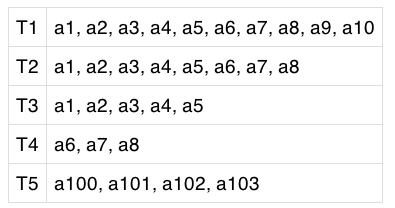
\includegraphics[width= 2.5in]{prob3.png}
	\begin{enumerate}[(1)]
		\item How many frequent patterns?
			\begin{homeworkSection}{Solution}
				2: a1, a2, a3, a4, a5 and a6, a7, a8
			\end{homeworkSection}
		\item What is the set of frequent closed patterns (list both pattern and support)? 			
			\begin{homeworkSection}{Solution}
				a1, a2, a3, a4, a5 support = 2/3\% and a6, a7, a8 support = 1\% \\
			\end{homeworkSection}
		\item What is the set of frequent max-patterns (list both pattern and support)? 
			\begin{homeworkSection}{Solution}
				a1, a2, a3, a4, a5 support = 2/3\% and a6, a7, a8 support = 1\% \\
			\end{homeworkSection}
		\item Show an example association rule that matches $(a1, a2, a3, a4, itemX) \rightarrow (itemY) [min\_support = 2, min\_confidence=70\%]$
			\begin{homeworkSection}{Solution}
  				
			\end{homeworkSection}
		\item For association rule $a1\rightarrow a6$, compute the following measures: confidence, lift, kulc.
			\begin{homeworkSection}{Solution}
  
			\end{homeworkSection}
		\item Among the above three measures, which ones are null-invariant? 
			\begin{homeworkSection}{Solution}
  
			\end{homeworkSection}
	\end{enumerate}
\end{homeworkProblem}
%=============================Problem4==========================%
\newpage
\begin{homeworkProblem}
	Given a database of four transactions $(min\_support = 2)$:\\
	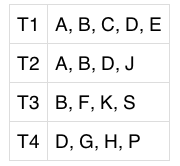
\includegraphics[width= 1.5in]{prob4.png}
	\begin{enumerate}[(1)]
		\item Show the major steps to find the frequent patterns using Apriori.
			\begin{homeworkSection}{Solution}
				\begin{enumerate}[(1)]
					\item The join step - first all transaction are scanned in order to count the number of occurrences of each item.  Next the support is computed equal to 50\%.  To discover the set of frequent 2-items $L_2$, the algorithm now uses the join.  
					\item The prune step - After completing the join step transactions are scanned and accumulated.  The set $C_2$ is now computed having minimum support.  
				\end{enumerate}
			\end{homeworkSection}
		\item Show the major steps to find the frequent patterns using FP-Growth (no need to draw the trees).
			\begin{homeworkSection}{Solution}
				\begin{enumerate}[(1)]
					\item The FP-tree is constructed - First scan the transaction database.  Collect frequency of items.  Next create the root of the FP-tree and label it as "null".    
					\item Mine the FP-tree by calling FP-Growth(FP-tree, null)  
				\end{enumerate}

			\end{homeworkSection}
		\item Compare the three algorithms: Apriori, FP-growth and ECLAT, by concisely discussing the major differences.  
			\begin{homeworkSection}{Solution}
				Both algorithms start by initially scanning all items in the database, however the algorithms largely differ when the analytical steps take place.  The major difference is the use joins in the Apriori algorithm whereas in the FP-Growth a tree structure is built.  
			\end{homeworkSection}
	\end{enumerate}
\end{homeworkProblem}

	
\end{spacing}
\end{document}

\begin{comment}%==========================================================
%=============================Problemi==========================%	
\begin{homeworkProblem}
	
	\begin{homeworkSection}{Solution}
		
	\end{homeworkSection}
\end{homeworkProblem}
%=============================Problemi==========================%	
\begin{homeworkProblem}
	
	\begin{enumerate}[(a)]
		\item 
			\begin{homeworkSection}{Solution}
		
			\end{homeworkSection}
	\end{enumerate}
\end{homeworkProblem}
%=============================Problemi==========================%	
\begin{homeworkProblem}
	{\bf }	
	\begin{homeworkSection}{Solution}
		
	\end{homeworkSection}
\end{homeworkProblem}
%=============================Problemi==========================%	
\newpage
\begin{homeworkProblem}
	{\bf  }	
	\begin{enumerate}[(a)]
		\item 
			\begin{homeworkSection}{Solution}
		
			\end{homeworkSection}
	\end{enumerate}
\end{homeworkProblem}
%=============================Problemi=========================%
\newpage
\begin{homeworkProblem}
	
	\begin{homeworkSection}{Solution}
		
	\end{homeworkSection}
\end{homeworkProblem}

\end{comment}%=========================================================
















